%
% This is a borrowed LaTeX template file for lecture notes for CS267,
% Applications of Parallel Computing, UCBerkeley EECS Department.
% Now being used for CMU's 10725 Fall 2012 Optimization course
% taught by Geoff Gordon and Ryan Tibshirani.  When preparing 
% LaTeX notes for this class, please use this template.
%
% To familiarize yourself with this template, the body contains
% some examples of its use.  Look them over.  Then you can
% run LaTeX on this file.  After you have LaTeXed this file then
% you can look over the result either by printing it out with
% dvips or using xdvi. "pdflatex template.tex" should also work.
%
\documentclass[twoside]{article}
\usepackage{graphicx}
\usepackage{tikz}
\usepackage{mathpazo}
\usetikzlibrary{decorations.pathmorphing}


\setlength{\oddsidemargin}{0.25 in}
\setlength{\evensidemargin}{-0.25 in}
\setlength{\topmargin}{-0.6 in}
\setlength{\textwidth}{6.5 in}
\setlength{\textheight}{8.5 in}
\setlength{\headsep}{0.75 in}
\setlength{\parindent}{0 in}
\setlength{\parskip}{0.1 in}
%
% ADD PACKAGES here:
%
\usepackage{amsmath,amsfonts,graphicx}
%
% The following commands set up the lecnum (lecture number)
% counter and make various numbering schemes work relative
% to the lecture number.
%
\newcounter{lecnum}
\renewcommand{\thepage}{\thelecnum-\arabic{page}}
\renewcommand{\thesection}{\thelecnum.\arabic{section}}
\renewcommand{\theequation}{\thelecnum.\arabic{equation}}
\renewcommand{\thefigure}{\thelecnum.\arabic{figure}}
\renewcommand{\thetable}{\thelecnum.\arabic{table}}
%
% The following macro is used to generate the header.
%
\newcommand{\lecture}[5]{
   \pagestyle{myheadings}
   \thispagestyle{plain}
   \newpage
   \setcounter{lecnum}{#1}
   \setcounter{page}{1}
   \noindent
   \begin{center}
   \framebox{
      \vbox{\vspace{2mm}
    \hbox to 6.28in { {\bf Physics 467/667: Thermodynamics/Statistical Physics
	\hfill Spring 2017} }
       \vspace{4mm}
       \hbox to 6.28in { {\Large \hfill Lecture #1: #2  \hfill} }
       \vspace{2mm}
       \hbox to 6.28in { {\it Lecturer: #3 \hfill Scribes: #4} }
      \vspace{2mm}}
   }
   \end{center}
   \markboth{Lecture #1: #2}{Lecture #1: #2}
   \vspace*{4mm}
}
%
% Convention for citations is authors' initials followed by the year.
% For example, to cite a paper by Leighton and Maggs you would type
% \cite{LM89}, and to cite a paper by Strassen you would type \cite{S69}.
% (To avoid bibliography problems, for now we redefine the \cite command.)
% Also commands that create a suitable format for the reference list.
\renewcommand{\cite}[1]{[#1]}
\def\beginrefs{\begin{list}%
        {[\arabic{equation}]}{\usecounter{equation}
         \setlength{\leftmargin}{2.0truecm}\setlength{\labelsep}{0.4truecm}%
         \setlength{\labelwidth}{1.6truecm}}}
\def\endrefs{\end{list}}
\def\bibentry#1{\item[\hbox{[#1]}]}
%Use this command for a figure; it puts a figure in wherever you want it.
%usage: \fig{NUMBER}{SPACE-IN-INCHES}{CAPTION}
\newcommand{\fig}[3]{
			\vspace{#2}
			\begin{center}
			Figure \thelecnum.#1:~#3
			\end{center}
	}
% Use these for theorems, lemmas, proofs, etc.
\newtheorem{theorem}{Theorem}[lecnum]
\newtheorem{lemma}[theorem]{Lemma}
\newtheorem{proposition}[theorem]{Proposition}
\newtheorem{claim}[theorem]{Claim}
\newtheorem{corollary}[theorem]{Corollary}
\newtheorem{definition}[theorem]{Definition}
\newenvironment{proof}{{\bf Proof:}}{\hfill\rule{2mm}{2mm}}
% **** IF YOU WANT TO DEFINE ADDITIONAL MACROS FOR YOURSELF, PUT THEM HERE:
\newcommand\E{\mathbb{E}}
\begin{document}
%FILL IN THE RIGHT INFO.
%\lecture{**LECTURE-NUMBER**}{**DATE**}{**LECTURER**}{**SCRIBE**}
\lecture{12}{Engines and Refrigerators}{Qiang Zhu}{scribe-name1,2,3}
%\footnotetext{These notes are partially based on those of Nigel Mansell.}
% **** YOUR NOTES GO HERE:
% Some general latex examples and examples making use of the
% macros follow.  
%**** IN GENERAL, BE BRIEF. LONG SCRIBE NOTES, NO MATTER HOW WELL WRITTEN,
%**** ARE NEVER READ BY ANYBODY.

\section{Some useful equations} % Don't be this informal in your notes!
\begin{equation} \label{idealgas} PV = nRT = NkT \end{equation}
\begin{equation} \label{Avogadro} N = n \times N_A \end{equation}
\begin{equation} \label{PV-micro} PV = Nm{\overline v_x^2} = NkT\end{equation}
\begin{equation} \label{eqpartition} U_{thermal} = N \cdot f \cdot \frac{1}{2}kT \end{equation}
\begin{equation} \label{1stlaw} \Delta{U} = Q + W \end{equation}
\begin{equation} \label{work3} \Delta W = - P \Delta{V} \end{equation}
\begin{equation} \label{entropy} S = k \text{ln}\Omega \end{equation}
\begin{equation} dU = TdS - PdV  + \mu dN\end{equation}

\section{Heat Engines and Refrigerators}
A heat engine is any device that absorbs heat and converts part of that energy into work.
Unfortunately,only part of the enregy absored as heat can be converted to work. 
The reason is that the the heat, as it flows in, brings along entropy, which must somehow
to be disposed as waste. 

\begin{figure}[ht]
\centering
\begin{tikzpicture}[thick]
\draw (0, -2.0) -- ( 0, 2.0) -- (4, 2.0) -- (4,-2.0) -- (0,-2.0);
\draw (-1, 2.1) -- (-1, 3.6) -- (5, 3.6) -- (5, 2.1) -- (-1, 2.1);
\draw (-1,-2.1) -- (-1,-3.6) -- (5,-3.6) -- (5,-2.1) -- (-1,-2.1);

\node at (1.8,2.8) {Hot reservoir, $T_h$};
\node at (1.8,-2.8) {Cold reservoir, $T_c$};
\node at (-1, 0) {Engine};
\draw [->,line width=0.1cm] (4, 0) -- (5.5,0) node [right]{$W$};
\draw [->,line width=0.1cm] (2, 2) -- (2,1) node  [below]{$Q_h$};
\draw [->,line width=0.1cm] (2,-1) -- (2,-2) node [below]{$Q_c$};

\draw (10,-2.0) -- (10, 2.0) -- (14, 2.0) -- (14,-2.0) -- (10,-2.0);
\draw ( 9, 2.1) -- ( 9, 3.6) -- (15, 3.6) -- (15, 2.1) -- ( 9, 2.1);
\draw ( 9,-2.1) -- ( 9,-3.6) -- (15,-3.6) -- (15,-2.1) -- ( 9,-2.1);

\node at (11.8,2.8) {Hot reservoir, $T_h$};
\node at (11.8,-2.8) {Cold reservoir, $T_c$};
\node at ( 8.5, 0) {Refrigenator};
\draw [<-,line width=0.1cm] (14, 0) -- (15.5,0) node [right]{$W$};
\draw [<-,line width=0.1cm] (12, 2) -- (12,1) node [below]{$Q_h$};
\draw [<-,line width=0.1cm] (12,-1) -- (12,-2) node [below]{$Q_c$};

\end{tikzpicture}
\caption{The schemes of cold and heat engines.}
\end{figure}

The benefit of heat engine is the work produced, $W$. Let's define the efficiency $e$,
\begin{equation} e = \frac{W}{Q_h} \end{equation}
Because of 1st law,
\begin{equation} Q_h = Q_c + W \end{equation}
\begin{equation} e = \frac{Q_h-Q_c}{Q_h} = 1 - \frac{Q_c}{Q_h} \end{equation}

According to the 2nd law,
\begin{equation}    S2 >= S1              ~~~~~~\rightarrow~~~~~~~ 
       \frac{Q_c}{T_c} >= \frac{Q_h}{T_h} ~~~~~~\rightarrow~~~~~~~
       \frac{Q_c}{Q_h} >= \frac{T_c}{T_h} ~~~~~~\rightarrow~~~~~~~
\end{equation}
Therefore, we conclude
\begin{equation} e<=1-\frac{T_c}{T_h} \end{equation}


\section{Refrigenator}
The benefit of refridgenator is $Q_c$. Let's define the efficiency $e$,
\begin{equation} e = \frac{Q_c}{W} \end{equation}
Because of 1st law,
\begin{equation} Q_h = Q_c + W \end{equation}
\begin{equation} e = \frac{Q_c}{Q_h-Q_c} = \frac{1}{Q_h/Q_c-1} \end{equation}

According to the 2nd law,
\begin{equation}    S2 >= S1              ~~~~~~\rightarrow~~~~~~~ 
       \frac{Q_c}{T_c} >= \frac{Q_h}{T_h} ~~~~~~\rightarrow~~~~~~~
       \frac{Q_c}{Q_h} >= \frac{T_c}{T_h} 
\end{equation}
Therefore, we conclude
\begin{equation} e<=\frac{1}{T_h/T_c-1} \end{equation}

\section{The Carnot Cycle}
How to reach the ideal efficiency?\\
In order to avoid entropy's increase, we need to \\
1, keep $T_h$ = $T_\text{agas}$ and $T_c$ = $T_\text{gas}$ during heat transfer;\\
2, In the course of temperature drop from $T_h$ and $T_c$, we use adiabatic condition to avoid heat waste.
\begin{figure}[ht]
\centering
\begin{tikzpicture}[x=6cm, y=8cm]
\draw [->] (1.4, 0.5) -- (3.2, 0.5) node[below]{$V$};
\draw [->] (1.4, 0.5) -- (1.4, 1.3)  node[above]{$P$};
\draw [->, line width=0.05cm, blue, domain=1.67:2.0]  plot(\x, {  2.0/\x})           node[above, yshift=0.5cm] {isothermal};
\draw [->, line width=0.05cm, black,domain=2.00:3.0]  plot(\x, {2.639/((\x)^(1.4))}) node[above, yshift=0.2cm] {adiabatic};
\draw [->, line width=0.05cm, blue, domain=3.0:2.50]  plot(\x, {1.701/\x})           node[below, yshift=-0.2cm] {isothermal};
\draw [->, line width=0.05cm, black,domain=2.5:1.67]  plot(\x, {2.453/((\x)^(1.4))}) node[below, yshift=-0.9cm] {adiabatic};
\end{tikzpicture}
\caption{The Carnot cycle.}
\end{figure}

{\bf Exercises}\\
\begin{enumerate}
\item Why must you put an air conditioner in the window of a building, rather than in the middle of a room?
\item Can you cool off your kitchen by refrigenator door open?
\item Prove that if you had a heat engine whose efficiency was better than the ideal value, you could hook it up to an ordinary Carnot refrigernator without work input.
\end{enumerate}

\section{Homework}
Problem 4.2, 4.3, 4.7, 4.11, 4.12

\end{document}

